\documentclass{article}

\usepackage[T1]{fontenc}    %Schriftart des Dokumentes
\usepackage[british]{babel} %Dokumentensprache, hier Deutsch
\usepackage{amsmath, amssymb, stmaryrd} %mathematische Schriftzeichen
\usepackage{graphicx} %Einfügen von Grafiken
\usepackage{wrapfig}
\usepackage{bm}

\setlength{\parindent}{0pt} %Einrückung von Absätzen auf null gesetzt
\setlength{\parskip}{10pt} %Abstand zischen Absätzen auf 10pt gesetzt

\title{Experiment 12: Moment of Inertia}
\author{Matthias Kuntz}
\date{18.09.2023}

\begin{document}

\maketitle

%-------------------------EINLEITUNG-------------------------
\section{Introduction}

In this experiment we will get to know rotational motions and firstly determine the deflecting force of a rotating pendulum. Using this, we can calculate the moment of inertia of a irregular shaped plate placed on the rotating pendulum for different rotating axes.  

\subsection{Basics}

Analogous to linear motion, angular motion is a basic field of classic mechanics. By clever definitions, one can define appropriate terms and variables which function using completely analogous equations in comparison to angular motion. We can create the following overview showcasing the most important variables and equations of angular motion and their corresponding linear equivalents:

\begin{table}[!ht]
    \centering
    \begin{tabular}{ccc}
        \textbf{linear motion} & & \textbf{angular motion} \\ \\
        position $r$ [\text{m}] & ~ & angular displacement $\theta$ [\text{rad}] \\
        velocity $v$ [$\frac{\text{m}}{\text{s}}$] & ~ & angular velocity $\omega$ [$\frac{\text{rad}}{\text{s}}$] \\
        acceleration $a$ [$\frac{\text{m}}{\text{s}^2}$] & ~ & angular acceleration $\alpha$ [$\frac{\text{rad}}{\text{s}^2}$] \\
        mass $m$ [\text{kg}] & ~ & moment of inertia $J$ [\text{kg} $\cdot$ m$^2$] \\
        force $F$ [\text{N}] & ~ & torque $\tau$ [$\frac{\text{kg} \cdot \text{m}}{\text{s}^2}$] \\
        impulse $p$ [$\frac{\text{kg} \cdot \text{m}}{\text{s}}$] & ~ & angular impulse $L$ [$\frac{\text{kg} \cdot \text{m}^2}{\text{s}}$] \\
        kinetic energy $K$ [\text{J}] & ~ & rotational energy $R$ [\text{J}] \\ \\
         $F=-kr$ & Hooke's Law & $\tau = -D\theta$ \\
         $E=\frac{1}{2}kr^2+\frac{1}{2}mv^2$ & Energy & $E=\frac{1}{2}D\theta^2+\frac{1}{2}J\omega^2$ \\
         $T=2\pi\sqrt{\frac{m}{k}}$ & oscillation period & $T=2\pi\sqrt{\frac{J}{D}}$ \\
    \end{tabular}
\end{table}

The last three lines of the table show the first important equations used in this experiment, where $k$ and $D$ are constants identified as the deflecting force of the pendulum. Using Hooke's Law for angular motion as well as the general equation for the torque $\tau = -Fr$ gives us:

\begin{equation}
    \begin{split}
        -D \theta &= -F r \\
        \iff \theta &= \frac{1}{D} Fr = \frac{1}{D} \tau 
    \end{split}
\end{equation}

The second form in equation 1 will be important for the first part of this experiment, where we want to determine the value of $D$ for our setup.

In general, the moment of inertia $J$ can be calculated by the following formula:

\begin{equation}
    J = \int r^2 \cdot dm
\end{equation}

This integral can be quite difficult to solve, especially when dealing with irregular shapes. For a slim disk rotating around its axis of symmetry we get:

\begin{equation}
    J_s=\frac{1}{2}m_sr_s^2
\end{equation}

Where $m_s$ is the mass and $r_s$ the radius of the disk.

For objects not rotating around the axis through the centre of mass we can use the parallel axis theorem (Steiner's theorem) which states that if the moment of inertia regarding rotation around the centre of mass $J_c$ is known, we can calculate the moment of inertia for a parallel rotating axis at distance $d$ of the centre of mass axis as follows:

\begin{equation}
    J=J_c+md^2
\end{equation}

Moments of inertia are extensive properties, meaning when an additional object is placed upon a rotating one, their individual moments of inertia regarding the rotating axis add up. 

\newpage

If we take our rotating table's moment of inertia to be $J_t$ and the one of the disk as $J_s$, we can derive the following oscillation times from the equation given in the overview as well as the extensive properties:

\begin{equation}
    \begin{split}
        T_1 &= 2\pi\sqrt{\frac{J_t}{D}} \\
        T_2 &= 2\pi\sqrt{\frac{J_t + J_s}{D}} \\
    \end{split}
\end{equation}

By squaring and subtracting the two equations we get another way to determine the value of $D$:

\begin{equation}
    D=4\pi^2 \frac{J_s}{T_2^2 - T_1^2} = 2\pi^2 \frac{m_sr_s^2}{T_2^2 - T_1^2}
\end{equation}

\newpage

\subsection{Experiment Setup}

A sketch of the experiment setup is shown on the next page in the measurement protocol. 

We will start by mounting the aluminium disk with the angle-scale on top of the rotating pendulum. The disk has a hook at its circumference where we can fix a string to connect to the loading platform, which is suspended over the edge of the table using a wheel bearing. With this first setup we can determine the angular displacement of the disk in dependence of the weight loaded onto the platform.

After that we will mount the rotating table onto the pendulum which has a clamp to fix the two brass plates onto the table. We will measure the oscillation periods of first just the table and then with each of the two plates fixated such that their centre of mass is on the rotational axis. To find the centre of mass of the irregular shaped plate we use the knife edged bearing and try to balance it in two different orientations, which will be marked on a sticker applied to the plate. The intersection of the two lines gives the centre of mass.  

Lastly, we will fixate the irregular plate at different points away from the centre of mass and again record the oscillation period for each position.

%---------------VERSUCHSPROTOKOLL MIT MESSDATEN---------------
\newpage

\section{Measurement Protocol}

\includegraphics[width=\textwidth]{graphics/mess1.jpg}
\newpage
\includegraphics[width=\textwidth]{graphics/mess2.jpg}
\newpage
\addtocounter{table}{5}

%-------------------------AUSWERTUNG-------------------------
\section{Evaluation}

\subsection{Calculation of the Deflecting Force $D$}

Firstly, we will calculate the Deflecting Force $D$ using the measurements of the angular diplacement in relation to the loaded weights. As shown in equation 1 $D$ is determined as the inverse of the slope of the best fit graph in figure 1, where the measured angles $\theta$ are plotted as a function of the torque $\tau$, which is calculated using the following equation:

\begin{equation}
    \tau = -Fr
\end{equation}

Where $r$ is the radius of the disk and $F$ the tangential force exerted by the loaded platform. By using the given weight $m=40g$ of one weight piece on the loading platform and the measured diameter $d = (10,0\pm0,1)$cm, we can calculate the torques:

\begin{equation}
\begin{split}
    \tau_i &= -F_ir = -(mi) g \frac{d}{2} \\
    \Delta \tau_i &= -(mi) g \frac{1}{2} \cdot \Delta d
\end{split}
\end{equation}

Here, $i$ is the amount of weight pieces currently on the platform. Since we are only interested in the absolute values we disregard the $-$ and get:

\begin{equation}
    \begin{split}
        \tau_1 &= (0,01962 \pm 0,00020) \frac{\text{kg} \cdot \text{m}^2}{\text{s}} \\
        \tau_2 &= (0,0392 \pm 0,0004) \frac{\text{kg} \cdot \text{m}^2}{\text{s}} \\
        \tau_3 &= (0,0589 \pm 0,0006) \frac{\text{kg} \cdot \text{m}^2}{\text{s}} \\
        \tau_4 &= (0,0785 \pm 0,0008) \frac{\text{kg} \cdot \text{m}^2}{\text{s}} \\
        \tau_5 &= (0,0981 \pm 0,0010) \frac{\text{kg} \cdot \text{m}^2}{\text{s}} \\
        \tau_6 &= (0,1177 \pm 0,0012) \frac{\text{kg} \cdot \text{m}^2}{\text{s}} \\
    \end{split}
\end{equation}

Plotting these values against the angular displacement results in $D$ and its error $\Delta D$. It is important to convert the measured angles $\Delta \theta$ and $\Delta \theta_f$ from degrees to radians using $1^\circ = \frac{2\pi}{360}$ before calculating the slopes.

\begin{equation}
    \begin{split}
        D &= \left( \frac{\Delta \theta}{\Delta \tau} \right)^{-1} = 0,0232 \frac{\text{Nm}}{\text{rad}} \\
        \Delta D &= \left| D - \left( \frac{\Delta \theta_f}{\Delta \tau_f} \right)^{-1} \right| = 0,0012 \frac{\text{Nm}}{\text{rad}} \\ \\
        \implies \bm{D} &= \bm{(0,0232 \pm 0,0012)} \frac{\textbf{Nm}}{\textbf{rad}}
    \end{split}
\end{equation}

\begin{figure} [p]
    \centering
    \includegraphics[width=\textwidth]{graphics/yuhuh.pdf}
    \caption{angular displacement as a function of torque}
\end{figure}

\newpage

\subsection{Calculation of the deflecting force via the oscillation period}

Firstly, we will calculate the median values as well as their errors for the measured oscillation periods from tables 2 and 3 of the protocol. After dividing the measured time by the amount of oscillations measured we get the oscillation period, therefore its error is also the error of the measured time divided by the count. To determine the error of the median value, we add the squares of the error of the oscillation periods and the standard error of the mean and take the sums square root. The results are shown in table 6.

\begin{table}[!ht]
    \centering
    \begin{tabular}{c|c|c|c|c|c}
        \textbf{table of origin} & $\bm{T}$ [s] & $\bm{\Delta T}$ [s] & $\bm{\overline{T}}$ [s] & $\bm{\Delta \overline{T}_\sigma}$ [s] & $\bm{\Delta \overline{T}}$ [s] \\ \hline
         & 1,225 & 0,025 &  &  &  \\
        2 & 1,226 & 0,025 & 1,225 & 0,00017 & 0,025 \\
         & 1,225 & 0,025 &  &  &  \\ \hline
         & 1,667 & 0,025 &  &  &  \\
        3 & 1,662 & 0,025 & 1,663 & 0,0018 & 0,025 \\
         & 1,662 & 0,025 &  &  &  \\
    \end{tabular}
    \caption{calculation of the mean values of the oscillation periods}
\end{table}

Now we need to calculate the moment of inertia of our round brass plate $J_s$. We use equation 3 and our measured values $m_s = (542,0\pm0,5)$g and $r_s=(5,25\pm0,05)$cm and calculate the error via propagation:

\begin{equation}
    \begin{split}
        J_s &= \frac{1}{2}m_sr_s^2 = 0,747 \cdot 10^{-3} \text{kg} \cdot \text{m}^2 \\
        \Delta J_s &= \frac{1}{2} \sqrt{\left( r_s^2 \cdot \Delta m_s \right)^2 + \left( 2 m_s r_s \cdot \Delta r_s \right)^2} = 0,014 \cdot 10^{-3} \text{kg} \cdot \text{m}^2 
    \end{split}
\end{equation}

Now we can calculate a second value for $D$ using equation 6 and the previously calculated values. Again we use propagation to calculate the error:

\begin{equation}
\begin{split}
    D' &= 4\pi^2 \frac{J_s}{\overline{T}_2^2 - \overline{T}_1^2} = 0,0233 \frac{\text{Nm}}{\text{rad}} \\
    \Delta D' &= \frac{4\pi^2}{\overline{T}_2^2 - \overline{T}_1^2} \sqrt{(\Delta J_s)^2 + \left( \frac{2 J_s \overline{T}_1 \cdot \Delta \overline{T}_1}{\overline{T}_2^2 - \overline{T}_1^2} \right)^2 + \left( \frac{2 J_s \overline{T}_2 \cdot \Delta \overline{T}_2}{\overline{T}_2^2 - \overline{T}_1^2} \right)^2} \\
    &= 0,0020 \frac{\text{Nm}}{\text{rad}} \\ \\
    \implies \bm{D'} &= \bm{(0,0233 \pm 0,0020)} \frac{\textbf{Nm}}{\textbf{rad}}
\end{split}
\end{equation}

We can now compare this second value $D'$ to our first value $D$:

\begin{equation}
    \sigma = \frac{|D'-D|}{\sqrt{\Delta D'^2 + \Delta D^2}} = 0,04
\end{equation}

As shown, both values are well within each others error intervals and show an insignificant deviation.

We estimate the second value $D'$ to be slightly more accurate because of the higher amount of measurements taken for it and use it from now on.

\newpage

\subsection{Calculation of the moments of inertia}

To calculate the moment of inertia of the irregular shaped plate, we first need to calculate the moment of inertia of the table using equation 5 and its error using propagation:

\begin{equation}
    \begin{split}
        J_t &= \frac{\overline{T}_1^2}{4\pi^2} D' = 0,89 \cdot 10^{-3} \text{kg} \cdot \text{m}^2 \\
        \Delta J_t &= \frac{1}{4\pi^2} \sqrt{(2 \overline{T}_1 D' \cdot \Delta \overline{T}_1)^2 + (\overline{T}_1^2 \cdot \Delta D')^2} = 0,08 \cdot 10^{-3} \text{kg} \cdot \text{m}^2 
    \end{split}
\end{equation}

By inserting $J_t$ in the second equation in 5, we can calculate the moment of inertia $J_i$ of the irregular plate. We note that $\Delta T_3 = \frac{\Delta t}{20} = 0,025$s, since $T_3$ is calculated by dividing the measured time by 20.

\begin{equation}
    \begin{split}
        J_i &= \frac{T_3^2}{4\pi^2} D'- J_t = 0,0023 \text{kg} \cdot \text{m}^2 \\
        \Delta J_i &= \sqrt{\left( \frac{T_3}{2\pi^2} \right)^2 \left( \left( D' \cdot \Delta T_3 \right)^2 + \left( \frac{1}{2} T_3 \cdot \Delta D' \right)^2 \right) + \left( \Delta J_t \right)^2} \\
        &= 0,0003 \\ \\
        \implies \bm{J_i} &= \bm{(0,0023 \pm 0,0003) \textbf{kg} \cdot \textbf{m}^2}
    \end{split}
\end{equation}

Now, we can calculate the the moments of inertia of the irregular plate regarding the shifted rotating axes in two different ways, either using the same way as we just calculated $J_i$ or using the parallel axis theorem. For the second, we use equation 4 and propagation of error to create the following formulas:

\begin{equation}
\begin{split}
    J_{i_n} &= J_i + m_i d_n^2 \\
    \Delta J_{i_n} &= \sqrt{(\Delta J_i)^2 + (d_n^2 \cdot \Delta m_i)^2 + (2m_id_n \cdot \Delta d)^2}
\end{split}
\end{equation}

The index $n$ indicates the stepwise increase in distance $d$ from the centre of mass.

The results for all moments of inertia are shown in table 7.

\begin{table}[!ht]
    \centering
    \begin{tabular}{c|c|c|c}
        $\bm{d}$ [cm] & $\bm{T_4}$ [s] & \textbf{(eq. 5)} $\bm{J_{i_n}}$ [$\text{kg} \cdot \text{m}^2$] & \textbf{(Steiner)} $\bm{J_{i_n}}$ [$\text{kg} \cdot \text{m}^2$] \\ \hline
        $0,50 \pm 0,05$ & $2,341$ & $0,0023 \pm 0,0003$ & $0,0023 \pm 0,0003$ \\ 
        $1,00 \pm 0,05$ & $2,373$ & $0,0024 \pm 0,0003$ & $0,0024 \pm 0,0003$ \\ 
        $1,50 \pm 0,05$ & $2,3965$ & $0,0025 \pm 0,0003$ & $0,0025 \pm 0,0003$ \\ 
        $2,00 \pm 0,05$ & $2,4475$ & $0,0026 \pm 0,0003$ & $0,0026 \pm 0,0003$ \\ 
        $2,50 \pm 0,05$ & $2,5005$ & $0,0028 \pm 0,0003$ & $0,0027 \pm 0,0003$ \\ 
    \end{tabular}
    \caption{moments of inertia regarding parallel axes}
    \bigskip
\end{table}

We plot the results in a diagram where the calculated ${J_{i_n}}$ is a function of the distance squared $d^2$, shown in figure 2.

\begin{figure} [!hb]
    \centering
    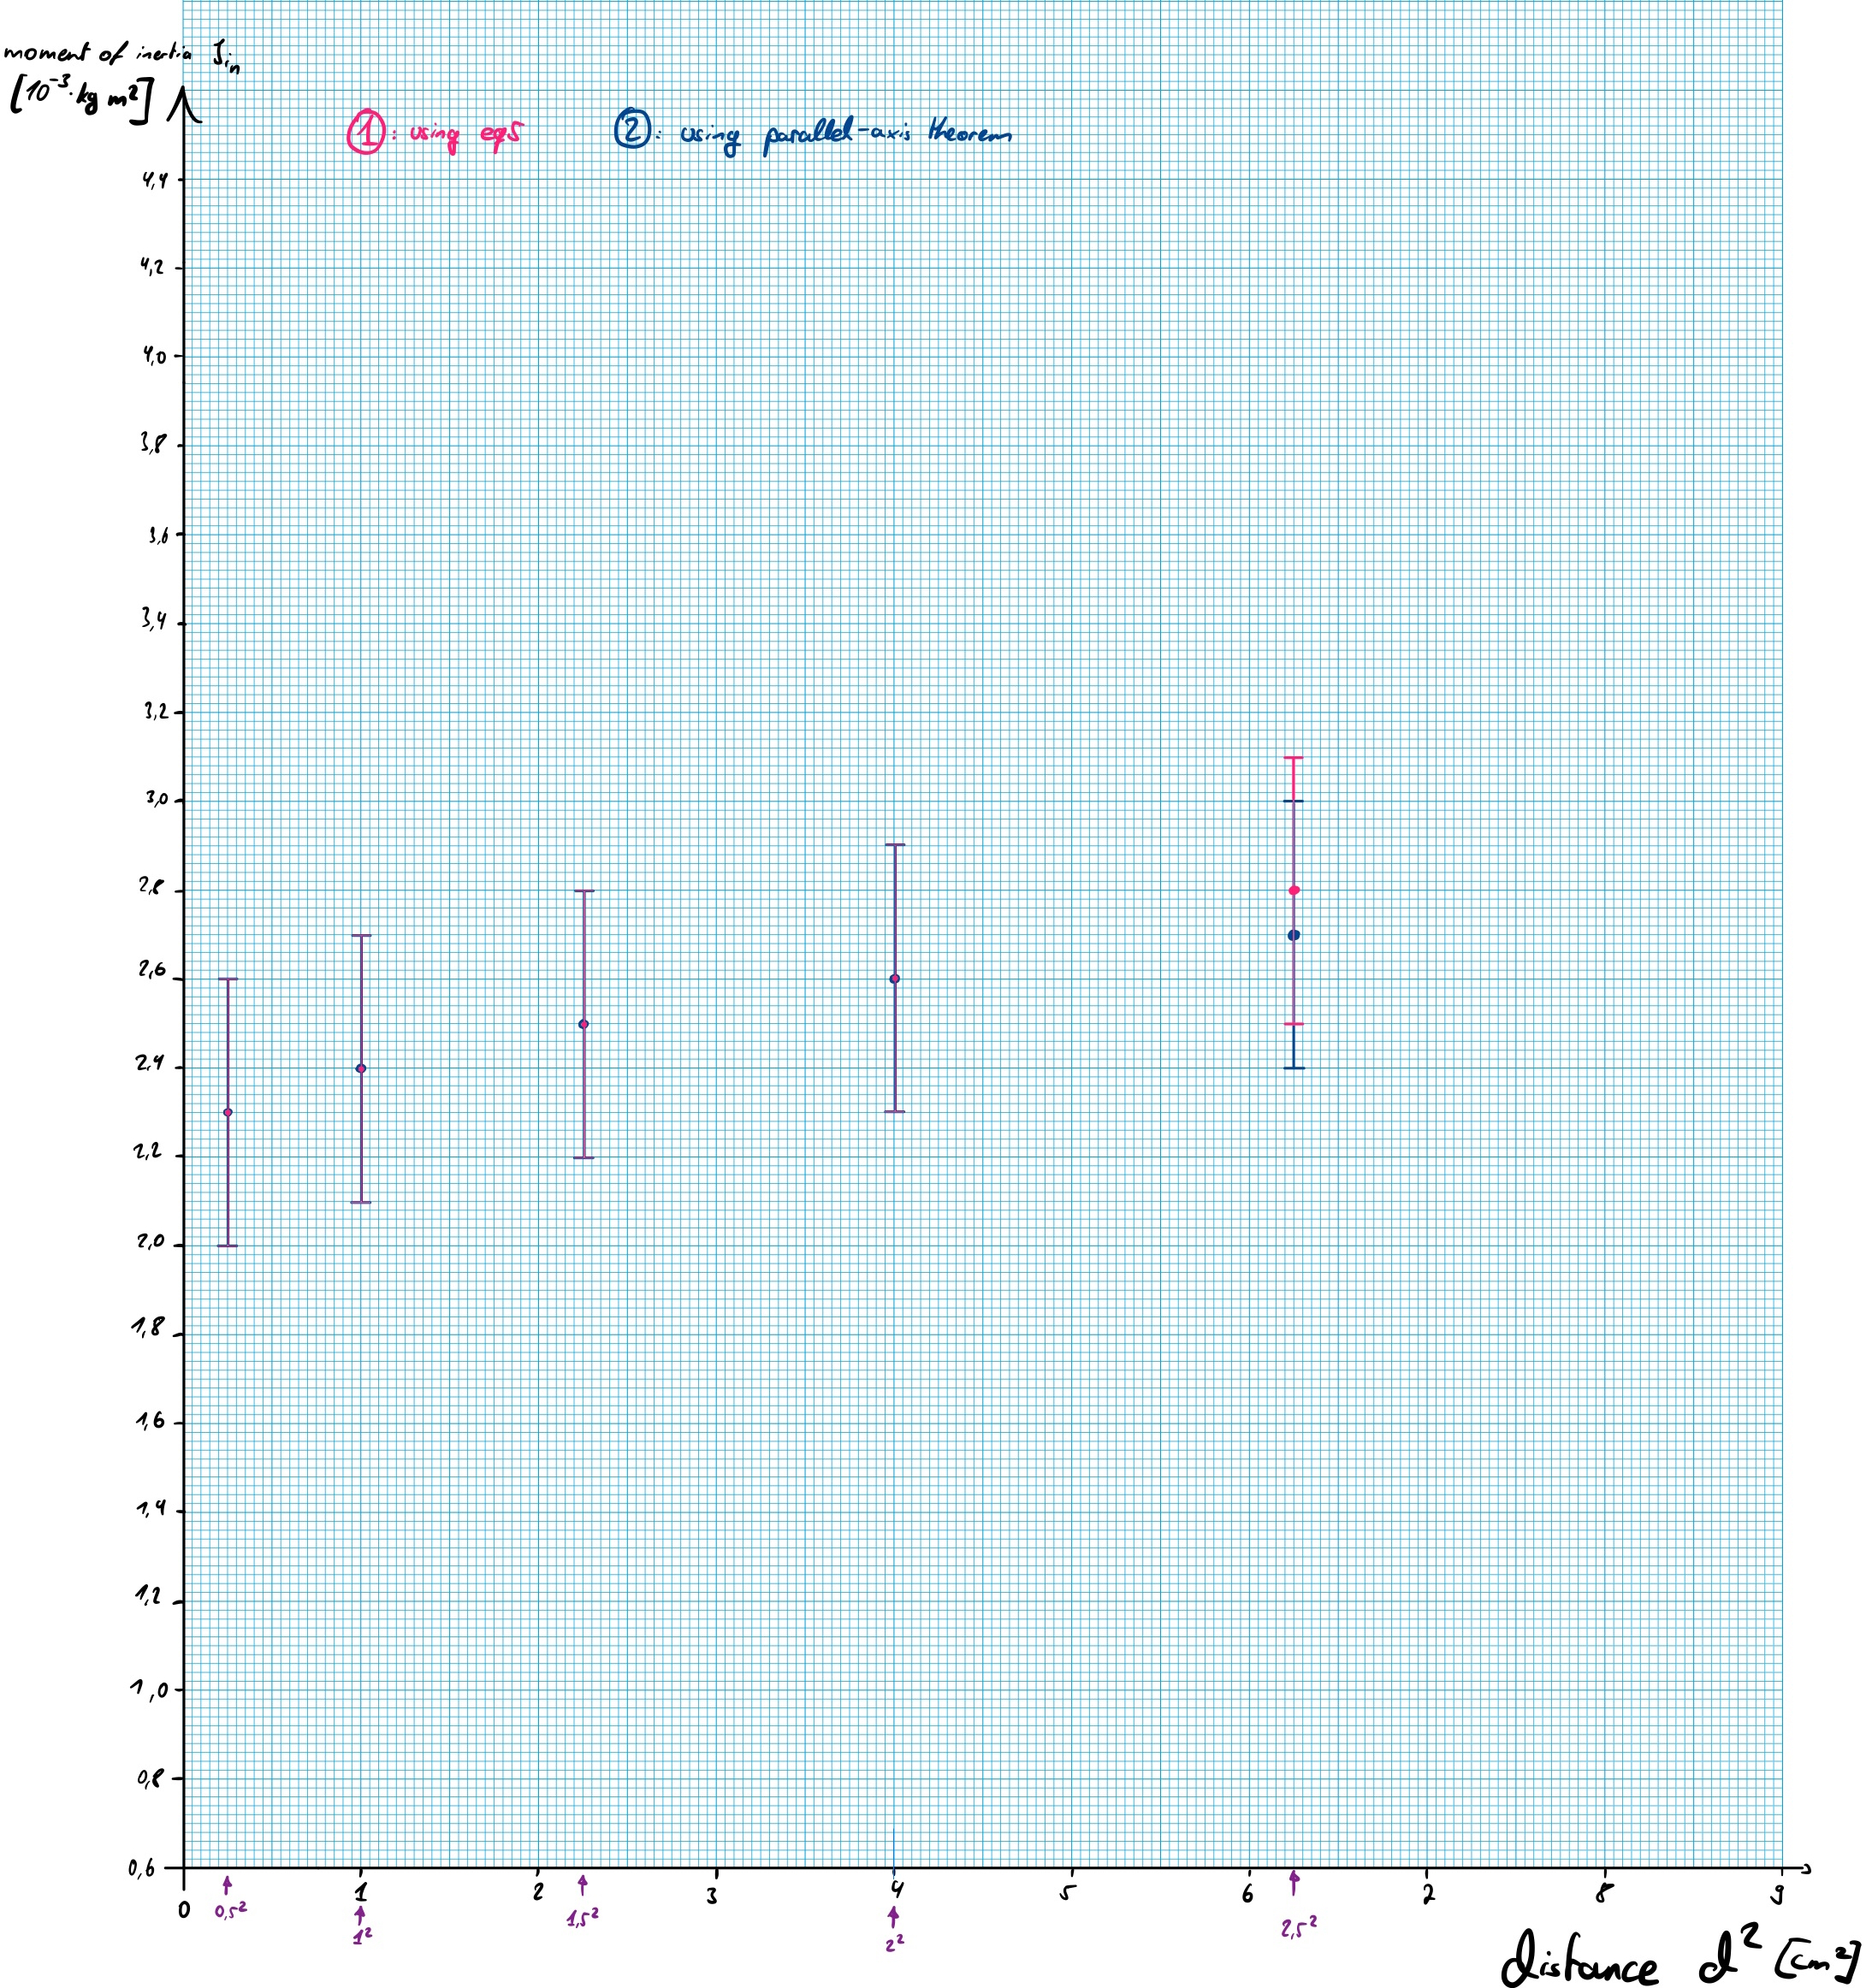
\includegraphics[width=\textwidth]{graphics/bruh.jpg}
    \caption{moments of inertia in comparison}
\end{figure}

\newpage
%---------------PRÄSENTATION DER ENDERGEBNISSE---------------
\section{Presentation of final results}

In this experiment we started by determining the deflecting force of our rotating pendulum by first measuring the angular displacement in relation to the applied weights on a loading platform connected to the perimeter of our oscillation table and secondly by recording the oscillation periods of an object with a known moment of inertia. The values we got were within insignificant sigma intervals of each other:

\begin{equation}
    \begin{split}
        \bm{D} &= \bm{(0,0232 \pm 0,0012)} \frac{\textbf{Nm}}{\textbf{rad}} \\
        \bm{D'} &= \bm{(0,0233 \pm 0,0020)} \frac{\textbf{Nm}}{\textbf{rad}}
    \end{split}
\end{equation}

Additionally, we calculated the moments of inertia of an irregular shaped brass plate regarding different rotating axes in two different ways, starting at the centre of mass and moving further outward. The following results were deducted:

\begin{equation}
        \bm{J_i} = \bm{(0,0023 \pm 0,0013) \textbf{kg} \cdot \textbf{m}^2}
\end{equation}

Using equation 5:

\begin{equation}
    \begin{split}
        \bm{J_{i_1}} &= \bm{(0,0023 \pm 0,0013) \textbf{kg} \cdot \textbf{m}^2} \\
        \bm{J_{i_2}} &= \bm{(0,0024 \pm 0,0003) \textbf{kg} \cdot \textbf{m}^2} \\
        \bm{J_{i_3}} &= \bm{(0,0025 \pm 0,0003) \textbf{kg} \cdot \textbf{m}^2} \\
        \bm{J_{i_4}} &= \bm{(0,0026 \pm 0,0003) \textbf{kg} \cdot \textbf{m}^2} \\
        \bm{J_{i_5}} &= \bm{(0,0028 \pm 0,0003) \textbf{kg} \cdot \textbf{m}^2} \\
    \end{split}
\end{equation}

Using Steiner's theorem:

\begin{equation}
    \begin{split}
        \bm{J_{i_1}} &= \bm{(0,0023 \pm 0,0003) \textbf{kg} \cdot \textbf{m}^2} \\
        \bm{J_{i_2}} &= \bm{(0,0024 \pm 0,0003) \textbf{kg} \cdot \textbf{m}^2} \\
        \bm{J_{i_3}} &= \bm{(0,0025 \pm 0,0003) \textbf{kg} \cdot \textbf{m}^2} \\
        \bm{J_{i_4}} &= \bm{(0,0026 \pm 0,0003) \textbf{kg} \cdot \textbf{m}^2} \\
        \bm{J_{i_5}} &= \bm{(0,0027 \pm 0,0003) \textbf{kg} \cdot \textbf{m}^2} \\
    \end{split}
\end{equation}

\newpage

%---------------ZUSAMMENFASSUNG UND DISKUSSION---------------
\section{Summary and Discussion}

In this experiment we calculated the deflecting force of our rotating pendulum using two different ways as well as the moments of inertia of an irregular shaped brass plate, also using two different ways.

A first notable observation would be, that all measured and calculated values showed expected results and were within error ranges and insignificant sigma intervals. The two determined values of the deflecting force were well within insignificant intervals with a sigma of $\sigma = 0,04$ and the calculated moments of inertia using the two different methods were also, apart from the last value which is off by 0,0001 digits, exactly the same. The calculated error values were also within reason, being at maximum 13\% of the calculated value, which is the case for the two $J_{i_1}$'s. Therefore, there are only some minor points to be addressed for further improvements.

During our experimentation, we had to determine the oscillation time by measuring 20 oscillations. To accurately measure one period there was a marking on the rotating table and an arrow on a stand, that could be used for orientation. The only problem being, that when we gave the pendulum a big enough starting amplitude to even distinguishably oscillate 20 periods, the clamp on the table would hit the arrow if it was put to close to it, meaning the arrow had to be at a further distance from the table somewhat diminishing the accuracy. 

Additionally, we need to mention the field of potential and easy errors when working with graphs per hand. Manually inserting points, finding best-fit as well as maximum-slope lines, and reading values off of diagrams is always faulty to some degree. Generally, the assistance of computer programs would have definitely given more accurate results, but still, our graphically determined value for the deflecting force was the value with the smallest relative error of all our calculated values with it being 5\% of the final result. Despite that, because of the general uncertainty when working with graphs per hand the value $D'$ was picked as the more accurate one and used for further calculations.

To conclude, despite the mentioned potential errors, all calculated values were determined within expected results and insignificant sigma intervals, which results in an all around satisfactory outcome.

\end{document}

